%!TEX root = ../main.tex
%=========================================================

\section{Performance Evaluation}
\label{sec:eval}
We implement \sysname in PeerSim~\cite{p2p09-peersim}, a large-scale peer-to-peer network simulator. We use an existing vanilla Kademlia implementation~\hl{[?]} as a starting point, extend it to make it equivalent to the existing Ethereum DHT a build \sysname on top of it. We compare our system against Discv4 (currently implemented in Ethereum) and a key/value store implemented on top Ethereum DHT (currently implemented in IPFS\hl{[]}), where advertisements are stored on the node closest to the topic hash. Similarly to current implementations of this solutions (\hl{[]}), we implement Last Recently Used advertisement replacement policy. 


We make the code publicly available for the scientific community\footnote{https://github.com/datahop/p2p-service-discovery}. In the evaluation, we focus on the following aspects: \textit{(1)} Optimal parameter selection, \textit{(2)} Overhead, \textit{(3)} Fairness and \textit{(4)} Security. 

\subsection{Evaluation Setup}

\begin{table}[!hbt]
\centering
\scriptsize
\begin{tabular}{|c|c|}%|c|c|}
\hline
Parameter     & Value (\%) \\
\hline
\hline
%Network size & 2000 nodes \\%&  0.4321 & 0.8883\\
%\hline
Simulation time & 4 hours \\%& 0.7569 & 0.9959\\
\hline
Kademlia bucket size & 16 \\%& 0.6104 & 0.8515\\
\hline
Kademlia buckets & 17 \\%& 0.8225 & 0.9897\\
\hline
Ticket table bucket size & 5 \\%& 0.8225 & 0.9897\\
\hline
Ticket table buckets & 10 \\%& 0.8225 & 0.9897\\
\hline
Lookup table bucket size & 16 \\%& 0.8225 & 0.9897\\
\hline
Lookup table buckets & 17 \\%& 0.8225 & 0.9897\\
\hline
Registration lifetime & 15 minutes \\%& 0.8225 & 0.9897\\
\hline
Registration waiting time limit & 15 minutes \\%& 0.8225 & 0.9897\\
\hline
Number of topics & 5 \\%& 0.8225 & 0.9897\\
\hline
Number of topics & 5 \\%& 0.8225 & 0.9897\\
\hline
Zipf dist exp & 0.7 \\%& 0.8225 & 0.9897\\
\hline
Ticket table capacity & 500 \\
\hline
Turbulence event & Every 144 seconds per 1000 nodes. \\%& 0.8225 & 0.9897\\
\hline
Num of connections & 50 \\%& 0.8225 & 0.9897\\
\hline
\bottomrule
\end{tabular}
\vspace{2mm}
\caption{Evaluation scenario parameters}
\label{tab:param}
\vspace{-0.05in}
\end{table}
\michal{In this section we need to justify our parameters}
In Table~\ref{tab:param} we show the parameters used in the simulation. 
We performed 4 hours long simulations with different number of nodes from 500 to 10000.
In the simulations there are 5 different topics and all nodes participate in at least one topic (t1).\michal{We need simulations with more topics. 5 is just not enough.}
There is turbulence in the simulation,  \ie new nodes are added to the network and existing nodes are removed at a rate of one event every 144 seconds per each thousand nodes in the network.\michal{Why 144? Do we have any churn data from Ethereum?}
Nodes are modelled similarly to an Ethereum client. 
When a node joins the network it starts advertising for the participating topics.
Each node has a pool of connections (separated by outgoing and incoming connections) for each topic in which they participate, and it perform lookups
for a specific topic to start connections with discovered nodes.
When an initial lookup is done,  the discovered nodes are stored in a buffer per topic.
Nodes start attempting connections with the discovered nodes from the buffer until all connections  are full.
In case the connection is possible (the targeted node has an available slot in the pool of connections and the node is still up), it is added 
to the local list of connections.
Nodes are removed from the discovered nodes buffer for each attempt of connection.
When a node goes down, a connection attempt is made with a new nodes from the buffer to occupy all available connection slots.
When the discovered nodes for a certain topic is empty, a new topic lookup is performed.
Nodes have a pool of 50 connections available, 16 for outgoing connections and 34 for incoming.
\michal{Should mention the Ethereum traces we use (Node IPs, IDs etc.)}
%\begin{table}[!hbt]
%\centering
%\scriptsize
%\begin{tabular}{|c|c|}%|c|c|}
%\hline
%Topic & 500 Nodes & 1000 Nodes & 5000 nodes & 10000 nodes \\
%\hline
%\hline
%T1 & 500 nodes & 1000 nodes & 5000 nodes & 10000 nodes \\%&  0.4321 & 0.8883\\
%\hline
%T2 & 1272 nodes \\%& 0.7569 & 0.9959\\
%\hline
%T3 & 803 nodes \\%& 0.6104 & 0.8515\\
%\hline
%T4 & 496 nodes \\%& 0.8225 & 0.9897\\
%\hline
%T5 & 218 nodes \\%& 0.8225 & 0.9897\\
%\hline
%\bottomrule
%\end{tabular}
%\vspace{2mm}
%\caption{Nodes per topic}
%\label{tab:nodes}
%\vspace{-0.05in}
%\end{table}
\michal{Should the Ethereum snapshots + IMC paper data be a base for the workloaded?}


\subsection{Parameter Selection}
\begin{figure}[!h]
\includegraphics[width=\linewidth]{img/placeholder}
\caption{Choose optimal parameter for $b$.} 
\label{fig:params_b}
\end{figure}

\begin{figure}[!h]
\includegraphics[width=\linewidth]{img/placeholder}
\caption{Choose optimal parameter for $P_\textit{occupancy}$.} 
\label{fig:params_b}
\end{figure}   

\begin{figure}[!h]
\includegraphics[width=\linewidth]{img/placeholder}
\caption{Choose optimal parameter for $P_\textit{ID}$ and   $P_\textit{IP}$.} 
\label{fig:params_b}
\end{figure}  

\begin{figure}[!h]
\includegraphics[width=\linewidth]{img/placeholder}
\caption{Choose optimal parameter for $P_\textit{topic}$.} 
\label{fig:params_b}
\end{figure}  


\subsection{Efficiency}
\michal{Do we just register here? Or also lookup? When a lookup is completed for all the solutions? Need to choose params for the Discv4}

\begin{figure}[!h]
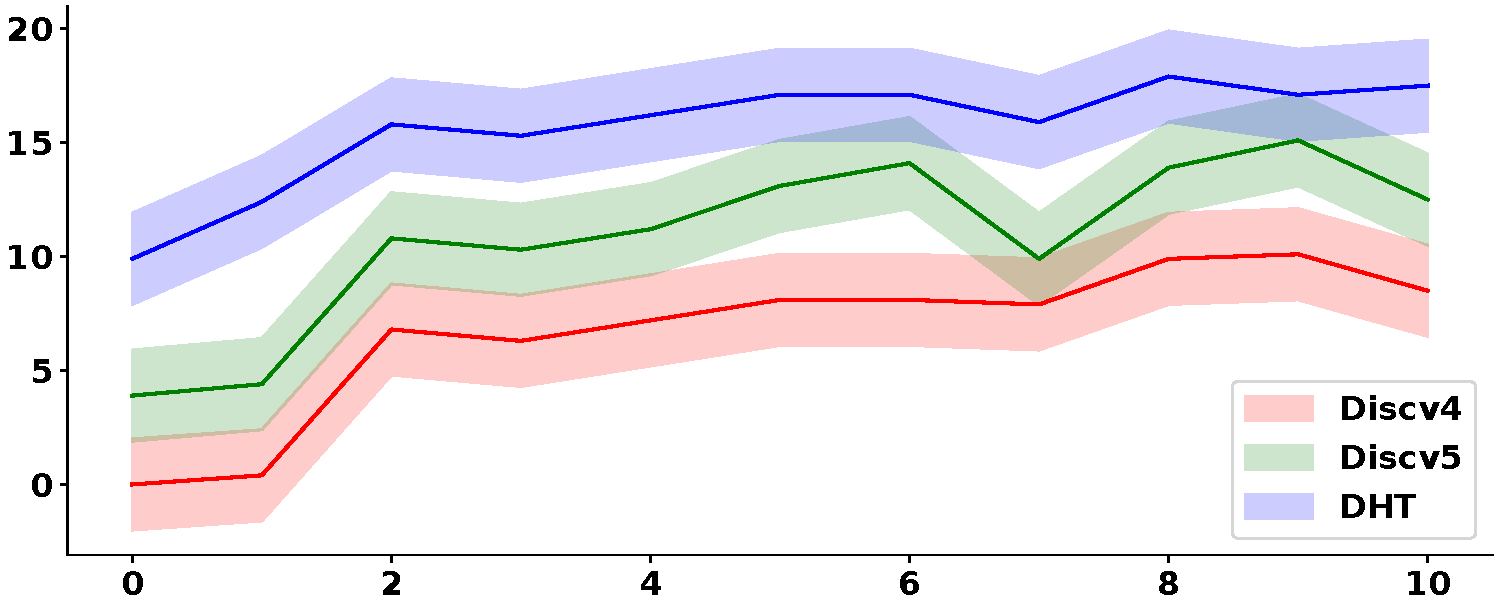
\includegraphics[width=\linewidth]{img/placeholder_max_min}
\caption{Y-axis: Messages sent/received per node (min, avg, max), X-axis: network size.} 
\label{fig:efficiency_messages_size}
\end{figure}

\begin{figure}[!h]
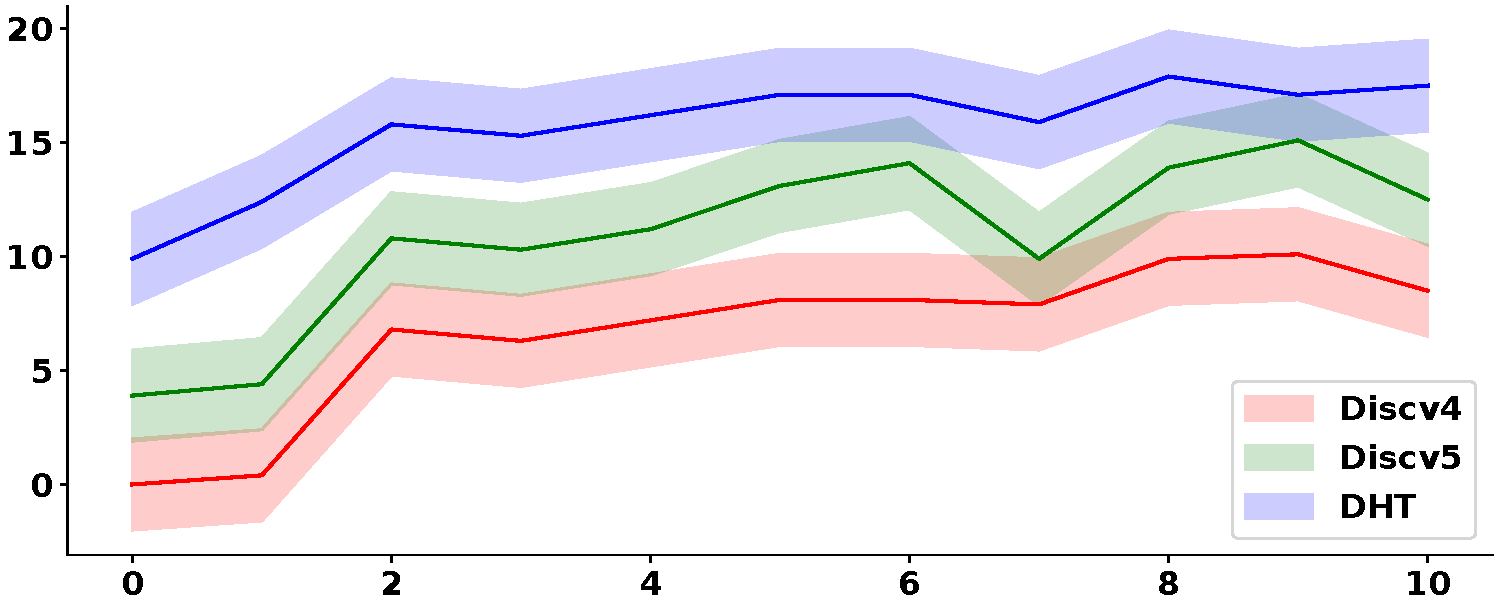
\includegraphics[width=\linewidth]{img/placeholder_max_min}
\caption{Y-axis: Messages sent/received per node (min, avg, max), X-axis: number of topics.} 
\label{fig:efficiency_messages_topics}
\end{figure}


\begin{figure}[!h]
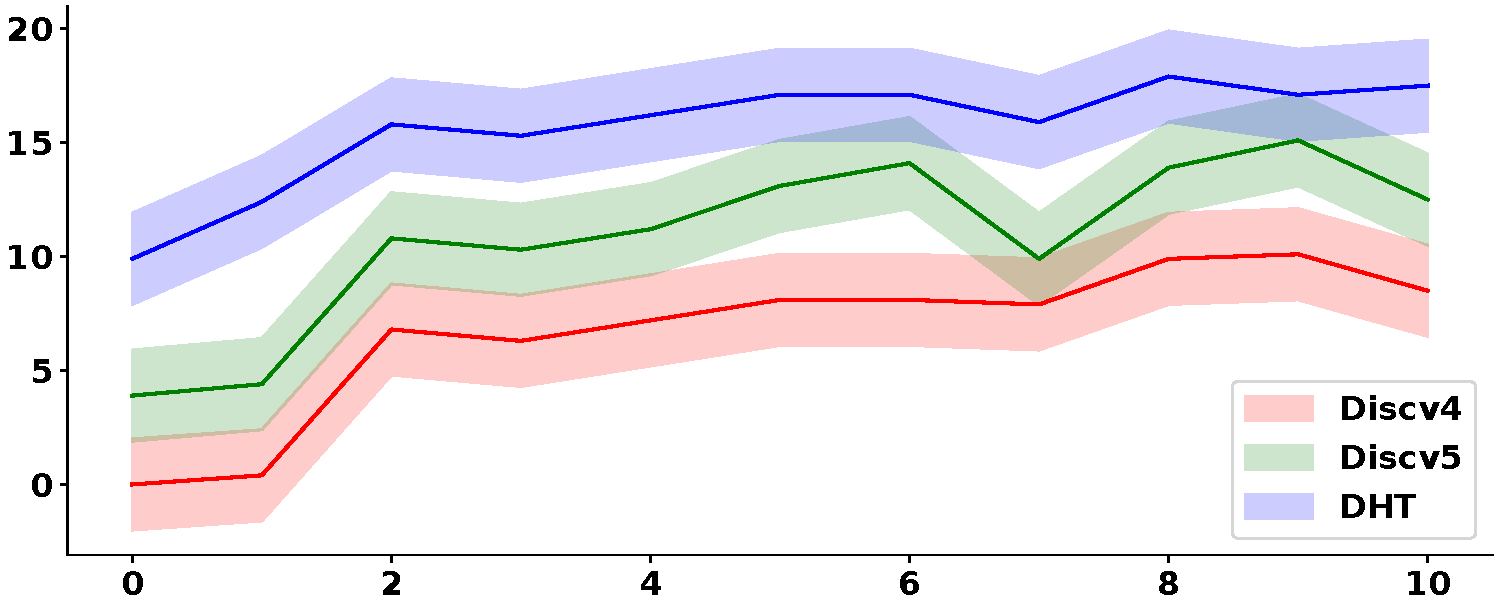
\includegraphics[width=\linewidth]{img/placeholder_max_min}
\caption{Y-axis: Messages sent/received per node (min, avg, max), X-axis: capacity of the table.} 
\label{fig:efficiency_messages_capacity}
\end{figure}


\subsection{Fairness}
\begin{figure}[!h]
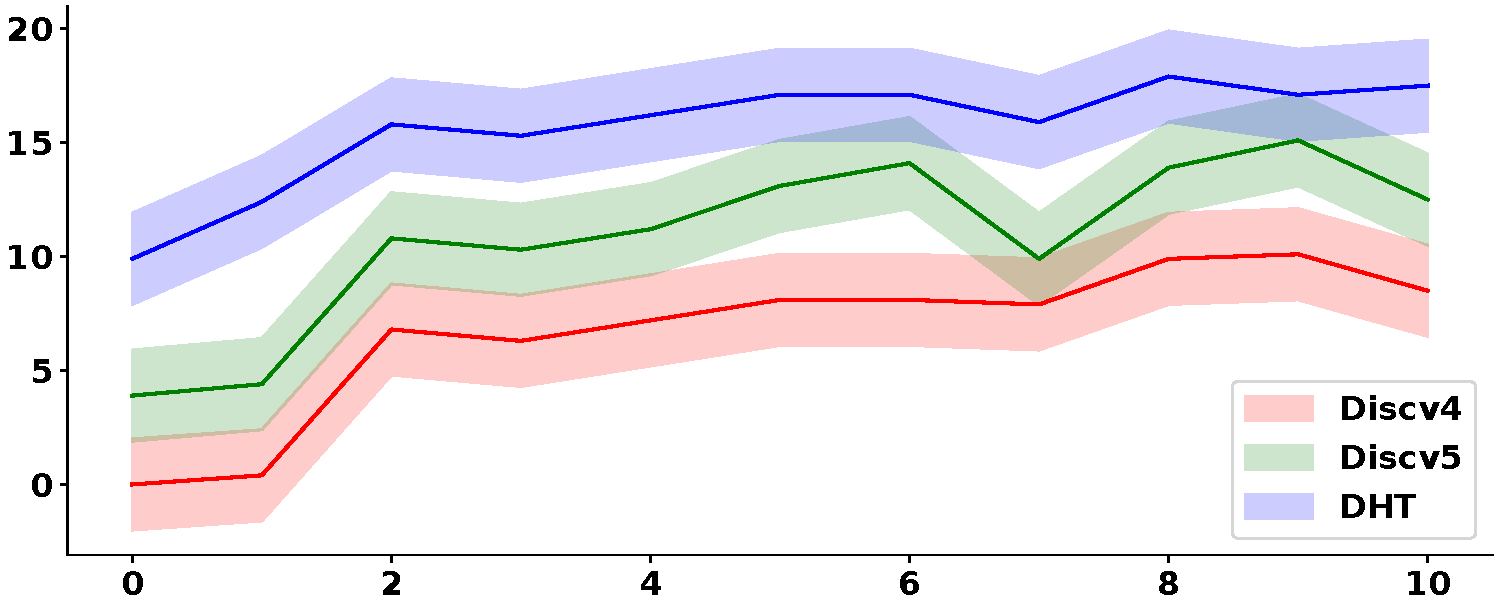
\includegraphics[width=\linewidth]{img/placeholder_max_min}
\caption{Y-axis: Time to register in [s] per topic (min, avg, max), X-axis: network size.} 
\label{fig:fairness_time_to_register_size}
\end{figure}

\begin{figure}[!h]
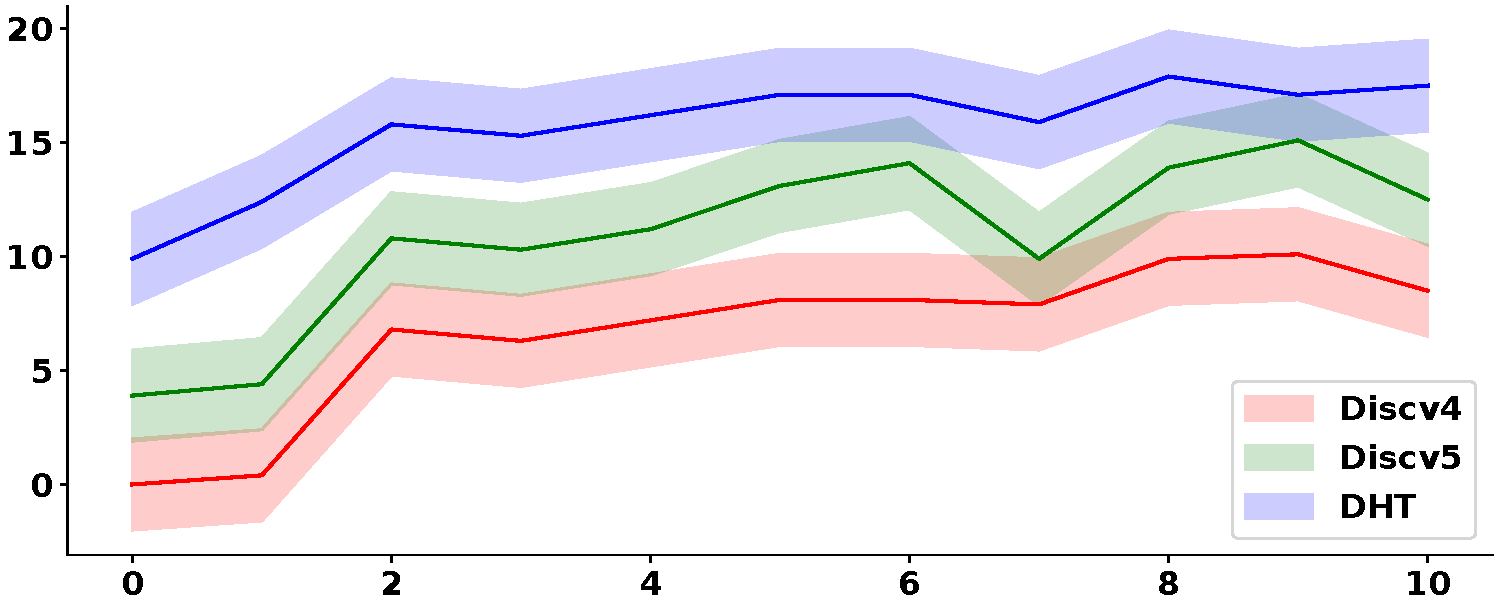
\includegraphics[width=\linewidth]{img/placeholder_max_min}
\caption{Y-axis: Time to register in [s] per topic (min, avg, max), X-axis: number of topics.} 
\label{fig:fairness_time_to_register_topics}
\end{figure}

\begin{figure}[!h]
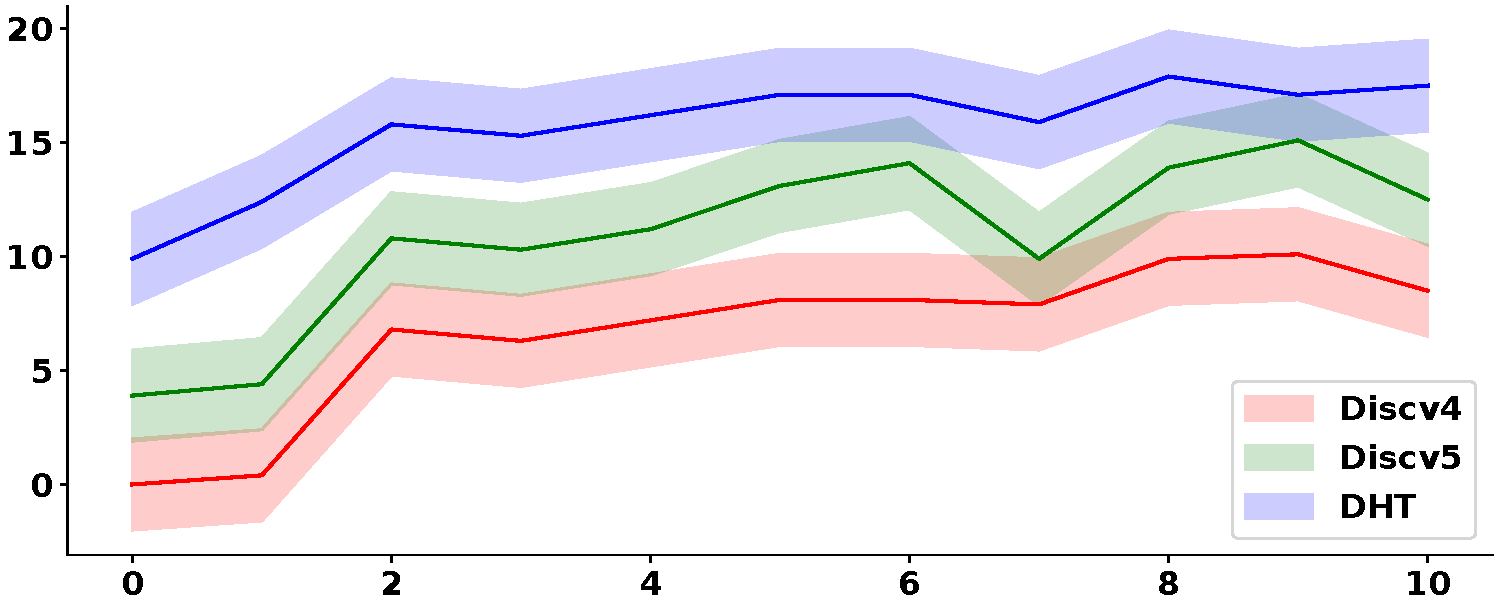
\includegraphics[width=\linewidth]{img/placeholder_max_min}
\caption{Y-axis: Time to discover in [s] per topic (min, avg, max), X-axis: network size.} 
\label{fig:fairness_time_to_discover_size}
\end{figure}

\begin{figure}[!h]
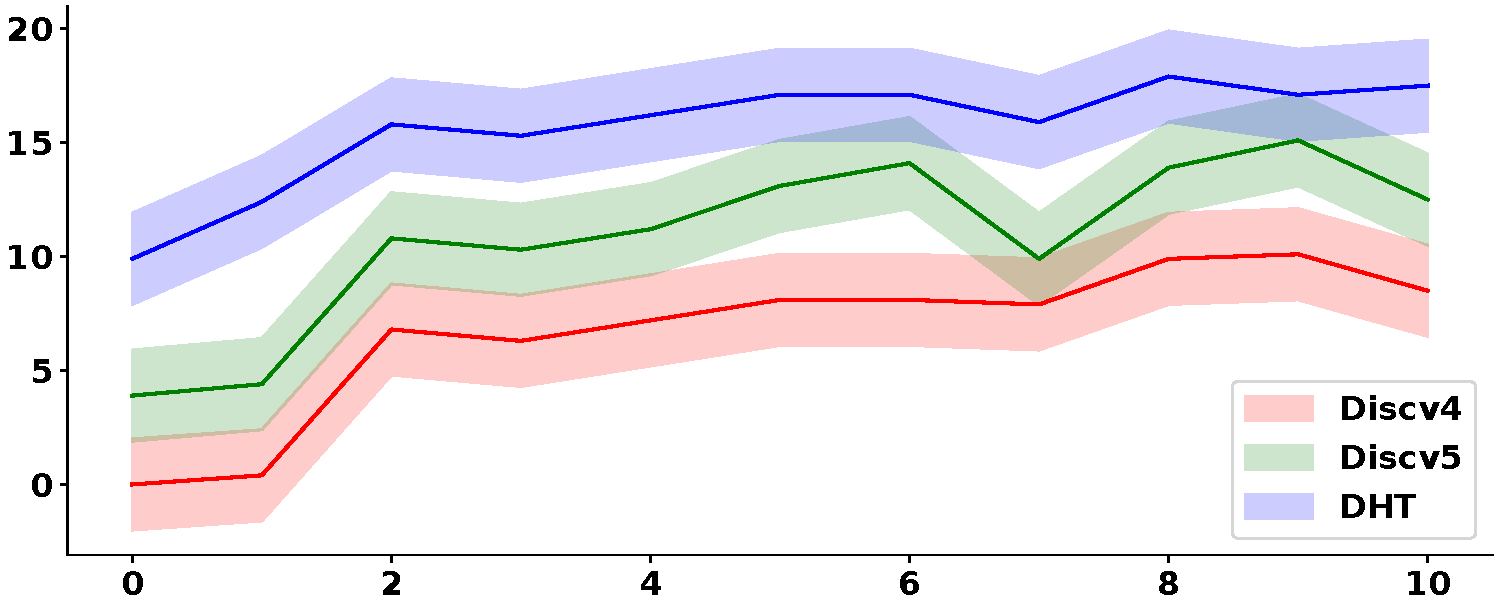
\includegraphics[width=\linewidth]{img/placeholder_max_min}
\caption{Y-axis: Time to discover in [s] per topic (min, avg, max), X-axis: number of topics.} 
\label{fig:fairness_time_to_discover_topics}
\end{figure}

\begin{figure}[!h]
\includegraphics[width=\linewidth]{img/placeholder}
\caption{How to show how many times each advertiser is being discovered?} 
\label{fig:params_b}
\end{figure}


\subsection{Security}
We evaluate \sysname resistance to two groups of malicious attacks:
\begin{itemize}
    \item \textbf{Eclipse Attack} - the attacker tries to make a target node discover and connect to peers under the attacker's control. The attack succeeds when all the inbound and outbound connections of the target node are established with malicious peers. 
    \item \textbf{Denial of Service (DoS)} - the attacker tries to disturb protocol operations. The attack succeeds when service discovery is made impossible or significantly delayed for a group of benign nodes.  
\end{itemize}
The attacker may use a large but finite number of malicious nodes. Both attacks may target a single node or a group of nodes (\eg nodes participating in a specific application). 

\para{Eclipse Attack}

\para{DoS Attack}
We implement and evaluate two kind of DoS attacks:
\begin{itemize}
    \item \textbf{Registration spam} - the attacker targets a registrars and sends a large number of registrations requests. If successful, the attacker exhaust registrar's resources and prevent benign nodes from registering. 
    \item \textbf{Malicious registrar} - the attacker deploys its nodes playing the role of registrars that \textit{(i)} return maximum waiting times when asked for a ticket, \textit{(ii)} return an empty set when asked about a topic. If successful, the attacker prevents benign advertisers from registering \textit{(i)} and prevents benign searchers from discovering their peers \textit{(ii)}. 
\end{itemize}

\begin{figure}[!h]
\includegraphics[width=\linewidth]{img/placeholder}
\caption{Compare only against DHT here I guess? Y-axis a ratio of popular malicious and benign ads in the table for spam attack and topic-targeted attack within a single registrar. X-axis: to avoid showing different graphs for multiple malicious IPs/IDs/nodes we can have a fix ratio between them i.e., each 5 Sybils (or requests/s) have 1 IP and 2 ID, and increase this "attacker strength".} 
\label{fig:security_spam}
\end{figure}

\begin{figure}[!h]
\includegraphics[width=\linewidth]{img/placeholder}
\caption{Compare only against DHT here I guess? Y-axis a  time to discovery/registration (do we care about registration if lookup works?) slowdown compared to a non-attack scenario?Do we consider different placements of Sybils here (i.e., only bucket 1? Or spread evenly across all the buckets?). X-axis: to avoid showing different graphs for multiple malicious IPs/IDs/nodes we can have a fix ratio between them i.e., each 5 Sybils have 1 IP and 2 ID, and increase this "attacker strength".} 
\label{fig:security_spam}
\end{figure}



\iffalse
\subsection{Performance Results}
\michal{We should group the result so that they show achievement of specific goals that we described before}

%\paragraph{Ticket registrations:
In the following we detail the performance evaluation in four different subsections.  In the first we show the registration performance.  Secondly we show the traffic load and overhead of the designed mechanism.  Then we continue with the lookup and discovery performance and we finish with the security analysis.

\subsubsection{Registration  performance}

In Figure~\ref{fig:regs} we observe the average active registrations in the system per topic with different number of nodes in the simulation,  from 500 to 10000 nodes. 
We can observe nodes for all topics are able to place a substantial amount of registrations, even the less popular topics. 
As number of nodes increase in the network, we can observe the differences between registrations per topic are reduced. 
Actually, it can be observed the most popular topic (t1) is able to place less registrations than t2. 
This is caused by the fact that with more nodes trying to register for the same topic,  waiting times increase.
If the waiting time increases over the waiting time limit (in the simulations is set to 15 min),  the node cancels the registration and tries with a different nodes.
When cancellations happen it may lead to less active registrations, because it may end up with longer registration processes.
In our simulation we observe less registrations for t1 than t2  because t1 registrations waiting time go over the waiting time limit more often.

In Figure~\ref{fig:time_reg} we observe the average time necessary for a node to place a registration,  from 500 to 10000 nodes in the simulation.
We can observe that average registration time is always below 500 seconds and this is reduced for less popular topics and smaller networks. 
This figure does not include registration times for cancelled registrations.
\sergi{I think we should include failed/uncomplete registrations in the plot}

\begin{figure}[!h]
\centering
\subfigure[{Active registrations}]{
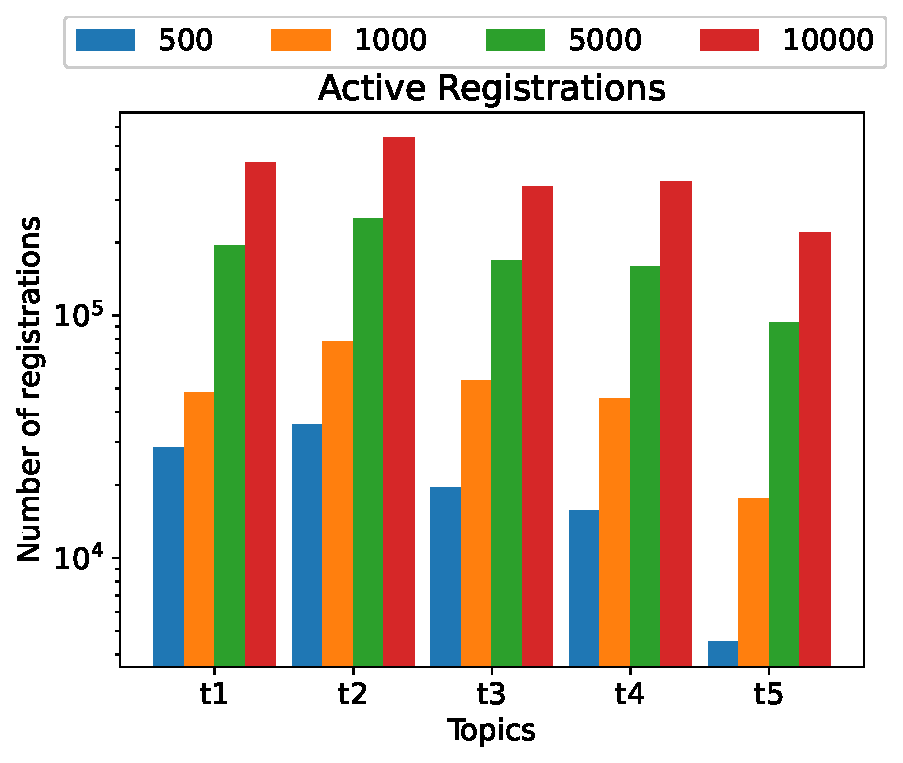
\includegraphics[width=0.225\textwidth]{img/eval/registration_origin.eps}
\label{fig:regs}
} 
\hspace{-0.25cm}
\subfigure[{Time to register}]{
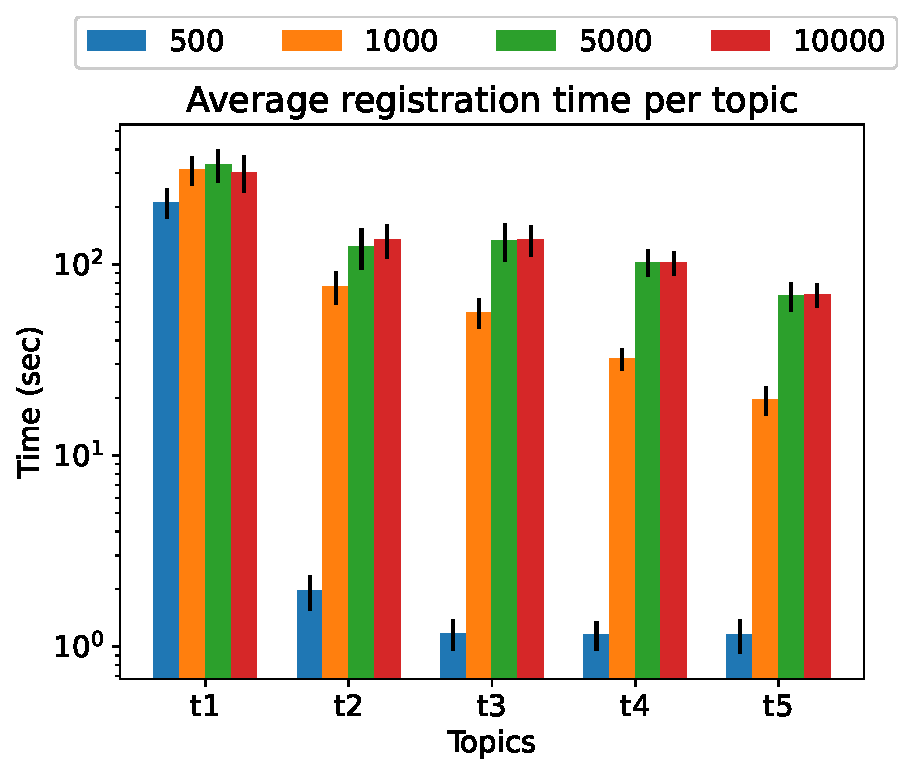
\includegraphics[width=0.225\textwidth]{img/eval/avg_time_register.eps}
\label{fig:time_reg}
}
 \caption{Ticket registrations} 
\label{fig:registrations}
\vspace{-0.15in}
\end{figure}   

%\begin{figure}[h!]
%\centering
%%\epsfig{file=imgs/eval/scen5.pdf, width=0.45\textwidth}
%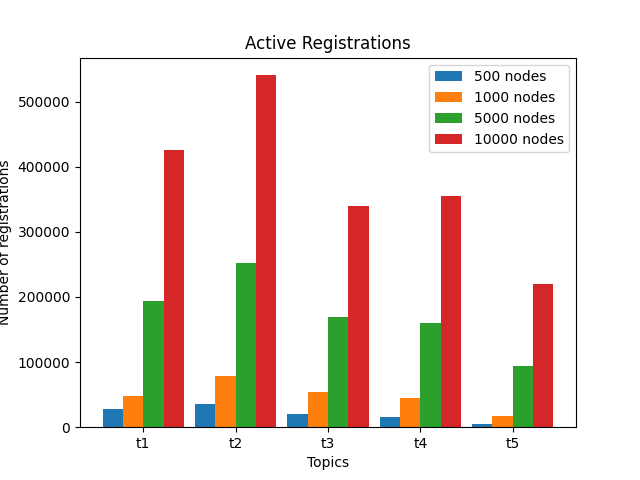
\includegraphics[width=0.225\textwidth]{img/eval/registration_origin.png}
%\caption{Registrations}
%\label{fig:regs}
%\vspace{-0.15in}
%\end{figure}

%\paragraph{\bf{Network load}:}
\subsubsection{Network load}

In Figure~\ref{fig:messages}~and~\ref{fig:msg_distr} we can observe the traffic load generated in the network.
In Figure~\ref{fig:messages} we observe most of the messages are ticket requests/replies, and the subsequent registration request/replies
after receiving a ticket from a node. 
This is caused by the fact that nodes are constantly registering dynamically. 
In Figure~\ref{fig:msg_distr} the messages received distribution. 
We can observe some nodes receive much more messages.
This is caused by the bucket node distribution, where nodes with identifiers close to topic hash ids receive more initial tickets requests because there are less.
However, we observe while the number of nodes in the network is increased 20 times,  the  maximum number of messages received by some nodes does not increase in the same way,  only being twice the amount when comparing 500 with 10000 nodes,  ans with increases lower than 30\% when number of nodes are doubled.
Moreover,  we can also see the number of messages received does not exceed 10 times the average value of the messages received. 

Therefore, the system is able to scale without danger of overloading some of the nodes of the network.

\begin{figure}[!h]
\centering
\subfigure[{Number of messages}]{
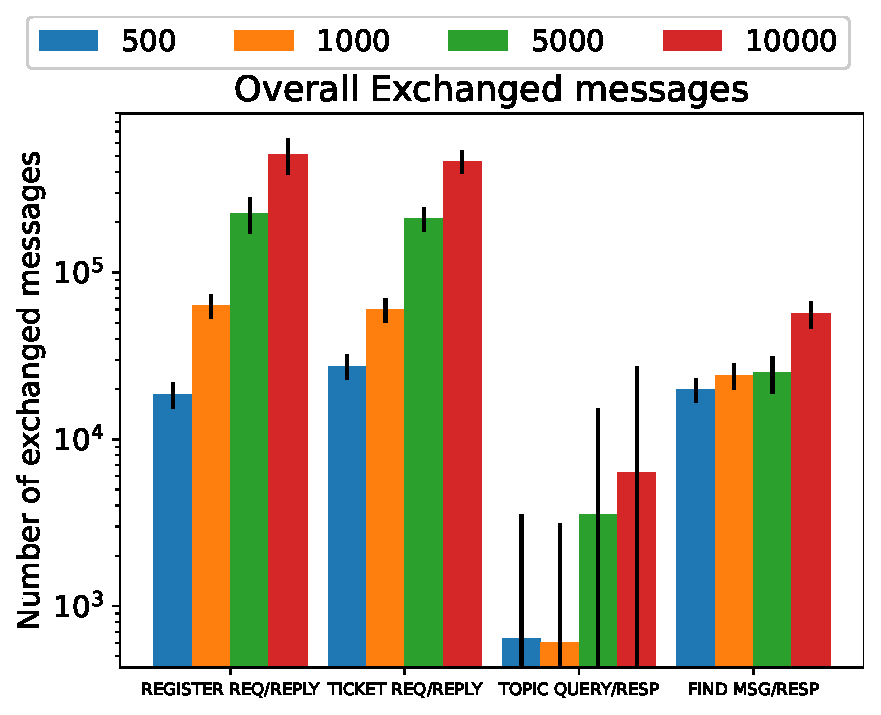
\includegraphics[width=0.225\textwidth]{img/eval/message_quantity.eps} 
\label{fig:messages}
} 
\hspace{-0.25cm}
\subfigure[{Message distribution}]{
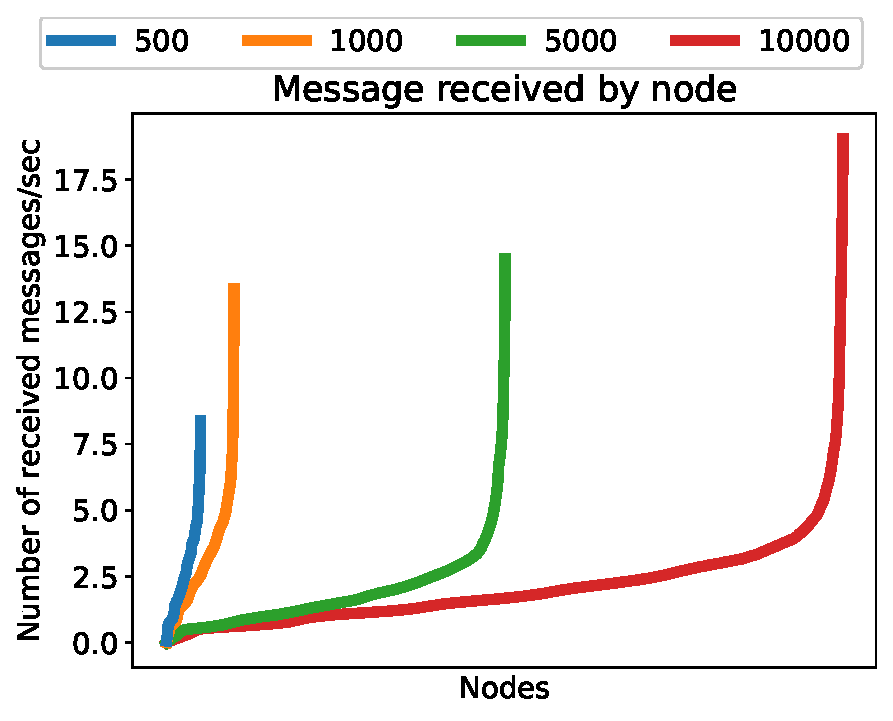
\includegraphics[width=0.225\textwidth]{img/eval/messages_received.eps} %\hspace{-1.5em}%
\label{fig:msg_distr}
}
 \caption{Traffic load} 
\label{fig:traffic}
\vspace{-0.15in}
\end{figure}   

\subsubsection{Discovery and lookup performance}

%\paragraph{\bf{Discovery performance}:}

In Figure~\ref{fig:reg_disc} and \ref{fig:timedisc} we can observe how nodes are discovered within the network.
In Figure~\ref{fig:reg_disc} we observe the percentage of the nodes in the network that are discovered and how often are discovered.
Each node in the network is represented by a circle, and the size of the circle represents the relative frequency of discoveries compared with other nodes in the network.
We can observe that for all topics the percentage of nodes discovered in the network is very close to 100\%. This means almost all nodes in the network are able to be discovered by other nodes. The number of discovered nodes is not 100\% because of the existence of turbulence (there are some nodes just joined the network and there has not been enough time yet to be discovered). In case there are a low number of nodes for a specific topic (e.g. t5 with 500 nodes network) the 100\% is reached.
We can also observe Figure~\ref{fig:reg_disc} that the discovery distribution is bounded to \hl{X} times between the most discovered and the least discovered.
We observe the dots size are very regular and despite being not completely equal the differences are not substantial. 
In Figure~\ref{fig:timedisc} we observe the time between a registration is completed and the first time the registration
is returned in a lookup.
By observing this we can see how difficult is for a node to be discovered once is able to place a registration. 
We see the average time is between 20 and 10 seconds in most of the cases, except for the least popular topic t5 which is around 50\% higher. 
We also observe the deviation is bounded at around 60 seconds, with equivalent different for t5.


\begin{figure}[!h]
\centering
\subfigure[{Registrant discovery distribution}]{
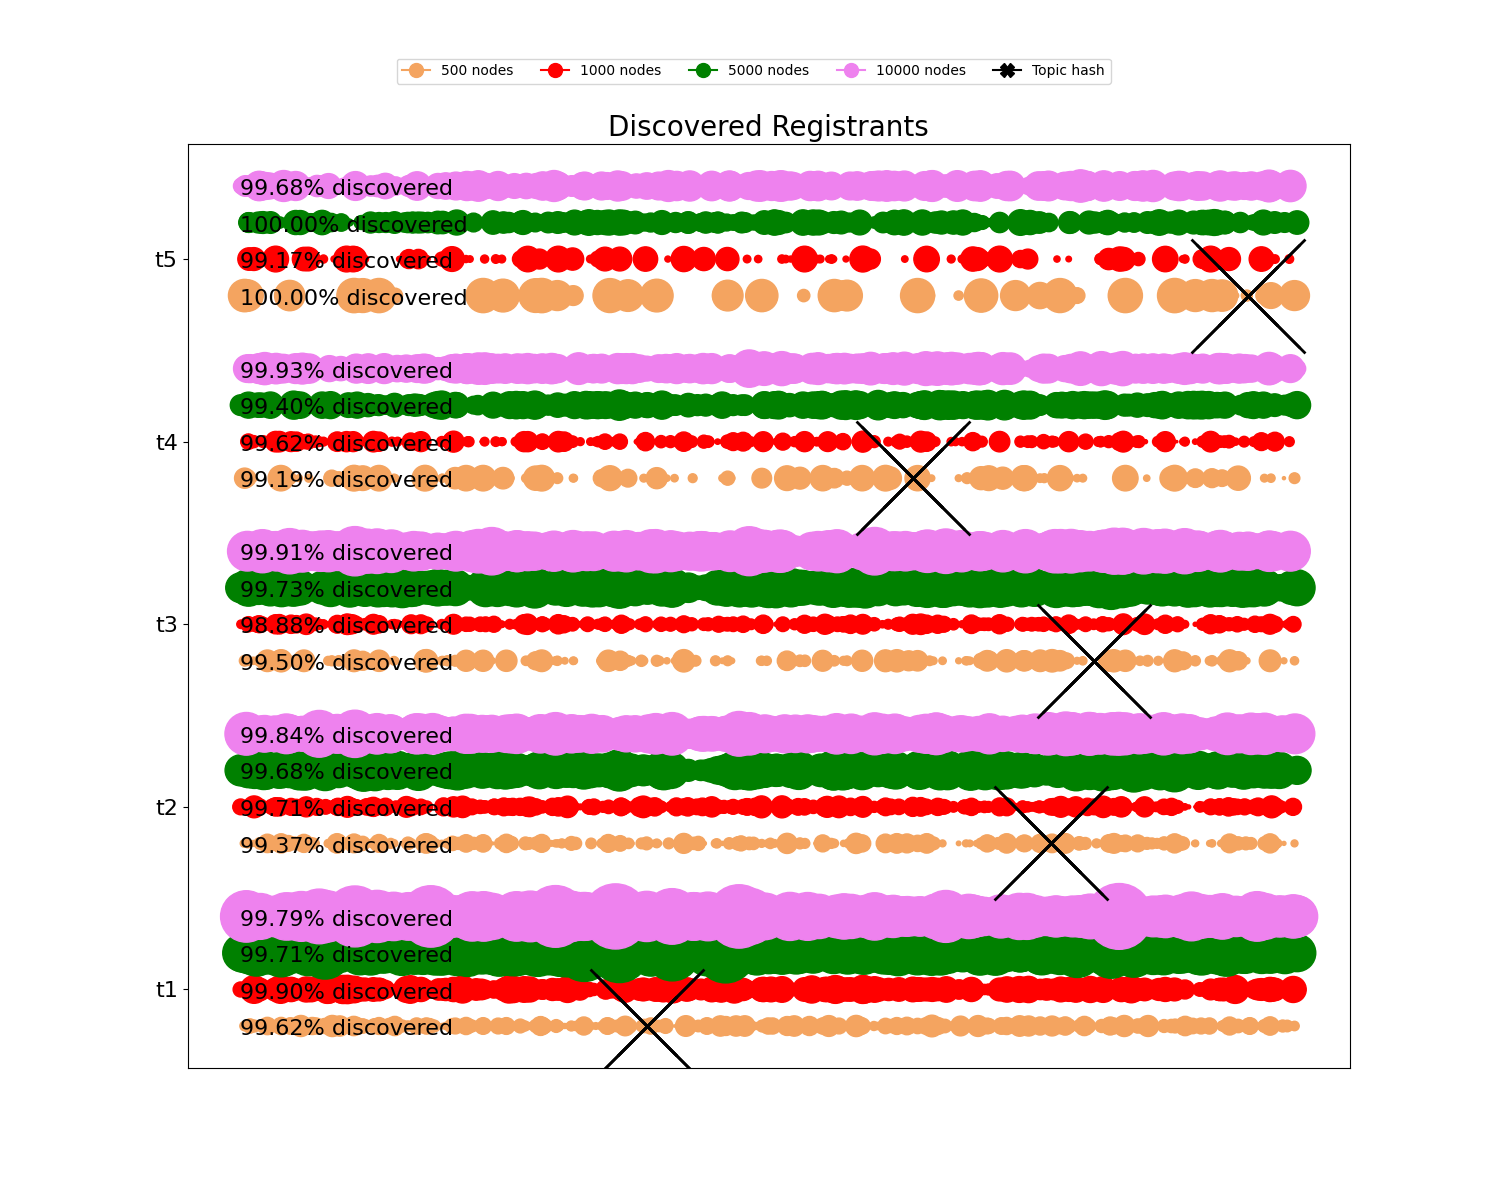
\includegraphics[width=0.225\textwidth]{img/eval/registrant_distribution.eps} 
\label{fig:reg_disc}
} 
\hspace{-0.25cm}
\subfigure[{Time between registration and first discovery}]{
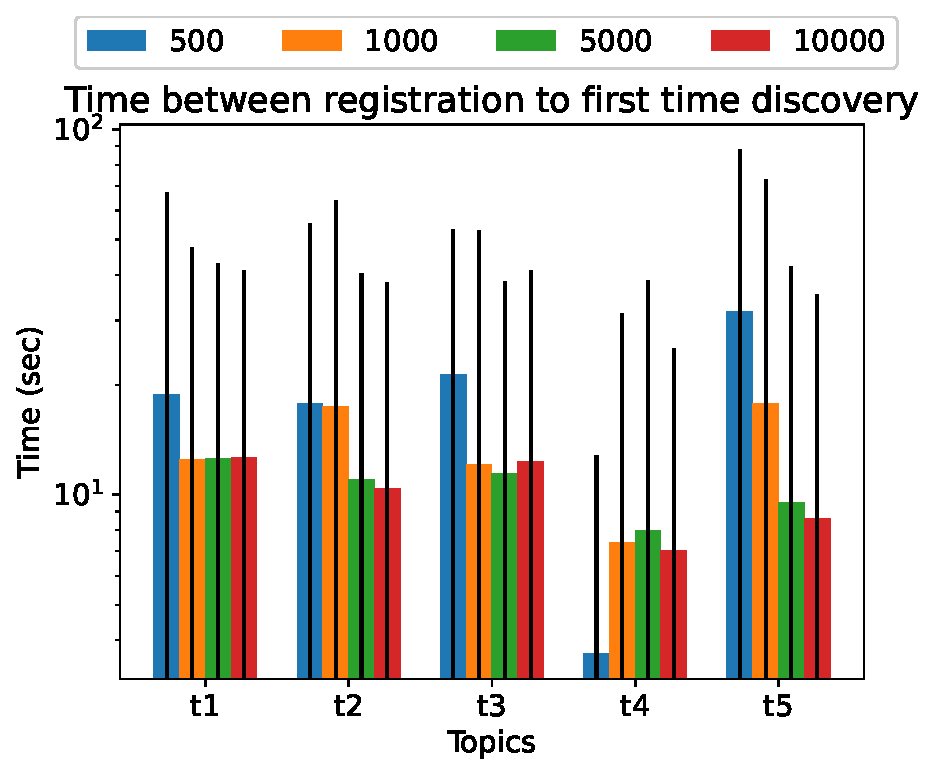
\includegraphics[width=0.225\textwidth]{img/eval/min_time_discovery.eps} %\hspace{-1.5em}%
\label{fig:timedisc}
}
 \caption{Discovery performance} 
\label{fig:discovery}
\vspace{-0.15in}
\end{figure}   


In Figure~\ref{fig:hopcount} we can observe the lookup performance of \sysname compared with Discv4 for a 5000 nodes simulation.
In the plot we show the average number of nodes discovered for each hop during a lookup per topic, taking into account that Discv4 cannot do per topic lookups,  so we discard received nodes that do not support the specific service.
In the figure we observe that for t1 the discovered nodes are higher when using Discv4, since all topics support t1 and any node discovered will be a valid node. 
However, as the popularity of the topic decreases it also does the lookup performance of Discv4,  since it is very difficult to find nodes for non-popular topics without supporting per topic lookups.
In this sense,  Discv5 lookup performance also decreases the performance with non-popular topics (simply because there are less nodes in the network) however this decrease is diminished.  Between t1 and t5 the lookup performance is decrease approximately to a 1/2th for Discv5, while when using Discv4 the lookup performance decreased to a less than a 1/10th.

%TODO add lookup description including mechanisms to avoid sybils.

\begin{figure}[h!]
\centering
%\epsfig{file=imgs/eval/scen5.pdf, width=0.45\textwidth}
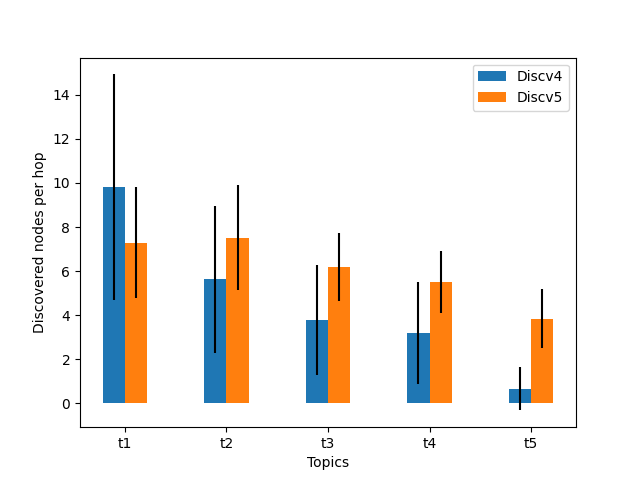
\includegraphics[width=0.35\textwidth]{img/eval/lookup_hopcount_discv4.png}
\caption{Lookup performance}
\label{fig:hopcount}
\vspace{-0.15in}
\end{figure}

\subsubsection{Sybil Attacks}

In the following we show the results of the performance evaluation of the discovery service under different sybil attacks.  The attacks that we evaluated in this section are of two types and are previously described in Section~\ref{sec:overview}. 
These attacks are eclipsing  and Denial-of-service (DoS) attacks.
Eclipsing attacks goal is to generate multiple fake identities within a topic to be able to eclipse existing nodes in the network.
Eclipsing a node imply all outbound and inbound connections are established to only sybil/fake nodes controlled by an attacker.
This allows the attacker to control the view of the network of the eclipsed node and can be used to co-opt a victim's mining power and use it to attack the blockchain's consensus algorithm.
DoS attacks instead is an attack meant to hamper the good performance or even to shut down the network, making it inaccessible to its intended users.  
In our case,  the goal of DoS attacks is to difficult or to block the discovery of nodes in the network and is specially important for topic with low popularity where finding all node in the network is very important.

In the implemented topic eclipsing attack,  malicious nodes are sybil nodes that cooperate in order to eclipse other valid nodes.
Malicious and valid nodes have the same amount of bandwidth resources and malicious nodes respond to topic lookup requests and find messages with only other malicious nodes.
Malicious nodes also act as evil 'registrants' trying to place as many registrations as possible by using bigger ticket size,  with malicious registrars attack,  where evil registrars replies with only malicious nodes when receiving a topic query.

We implemented and evaluated two kind of DoS attacks.  
The first attack consists in a topic spam attack where a big number of sybil identities generated try to register for non-existing random topics.
By registering for non-existing topics,  evil nodes try to harm valid topics registrations, overflowing topic tables.
The second DoS attack consists on generating sybil identities that keep without replying when receiving valid nodes ticket requests or return very long waiting times. 
This way an attacker can try to backlog valid nodes ticket registrations.

In Figures~\ref{fig:reg_eclipse},~\ref{fig:discoverytime_eclipse}~and~\ref{fig:lookup_eclipse} we show performance results under a
topic eclipsing attack.
We compare results for topic eclipsing attacks targeted to the most popular topic (t1) and attacks targeted to the least popular topic (t5). 
In the simulation there are 2000 nodes, all of them participating in t1 and only 218 participating in t5. 
In the simulations there are an additional 20\% (400 in total) malicious nodes that target the specific topic and the number of resources used in the attack (IP addresses) vary from 1 address to 50.

\begin{figure}[!h]
\centering
\subfigure[{Active registrations eclipse attack t1 attack}]{
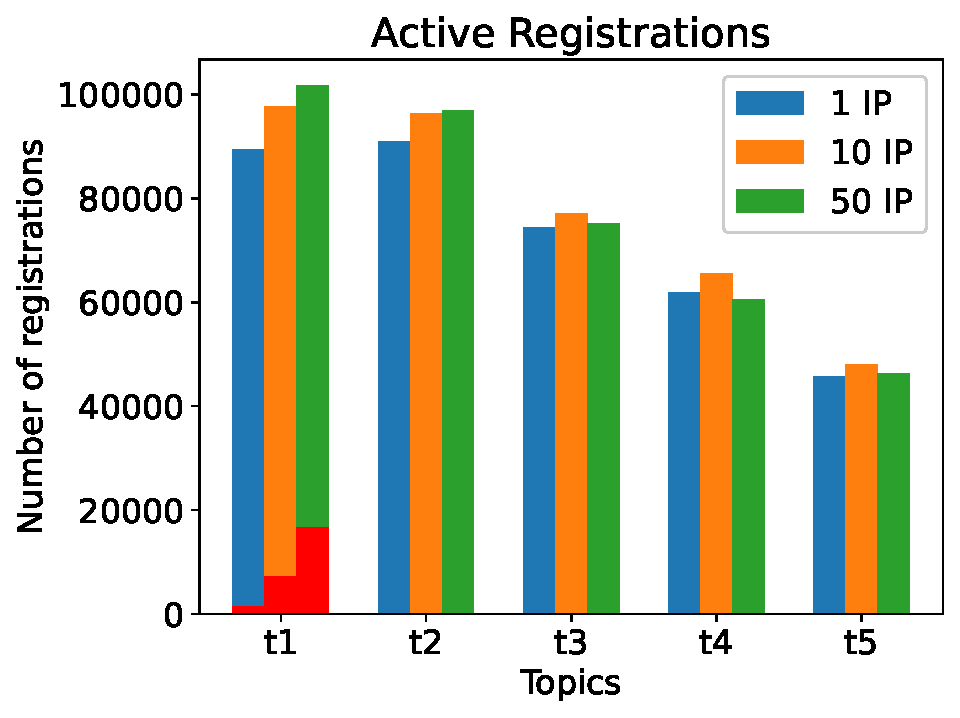
\includegraphics[width=0.22\textwidth]{img/eval/attack/registration_origin_t1.eps} 
\label{fig:reg_eclipse_t1}
} 
\hspace{-0.15cm}
\subfigure[{Active registrations eclipse attack t5 attack}]{
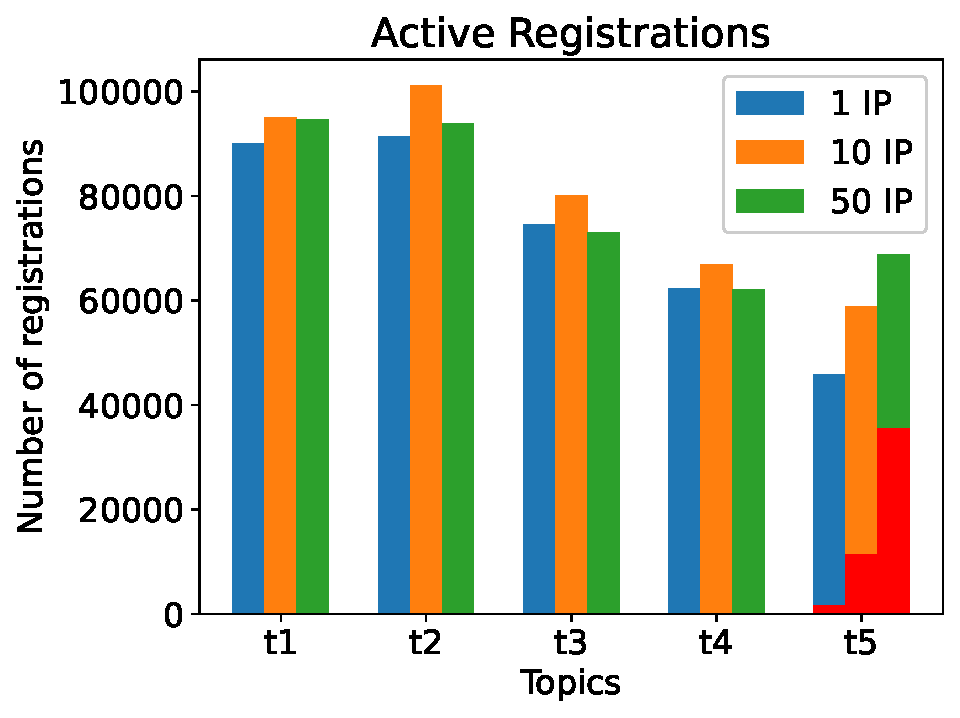
\includegraphics[width=0.22\textwidth]{img/eval/attack/registration_origin_t5.eps} %\hspace{-1.5em}%
\label{fig:reg_eclipse_t5}
}
 \caption{Active registrations under topic eclipsing attack} 
\label{fig:reg_eclipse}
\vspace{-0.15in}
\end{figure}   

In Figure~\ref{fig:reg_eclipse_t1} we observe the active registrations in the simulation per topic, for an eclipsing attack targeted to the most popular topic (t1), including active registrations of malicious nodes.
We can observe than even though the number of malicious nodes is equivalent to 20\%, the number of active registrations is lower than that. 
As expected, as the number of IP addresses used in the attack increaseas, the number of active registrations of malicious nodes also increase, since different malicious nodes with complete different IPs can not be diffierentiated from valid nodes.
For topic 5, the most vulnerable topic for being the least popular, we can observe a similar pattern of active registrations. 
However, we observe that despite malicious nodes being more (400 nodes) than valid nodes (218 nodes), active registrations of malicious nodes is kept lower than 30\% in all cases. Similarly to t1, the active registrations increase with the higher number of IPs used in the attack, since there is no way to a totally distributed attack without reusing IP addresses.


\begin{figure}[!h]
\centering
\subfigure[{Time between registration and first discovery t1 attack}]{
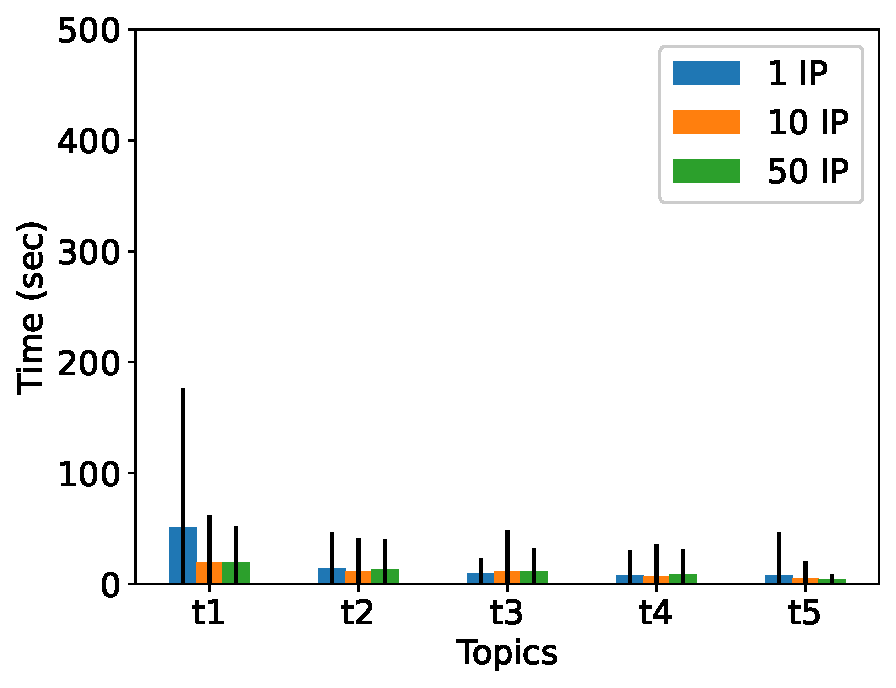
\includegraphics[width=0.225\textwidth]{img/eval/attack/min_time_discovery_t1.eps} 
\label{fig:discoverytime_eclipse_t1}
} 
\hspace{-0.16cm}
\subfigure[{Time between registration and first discovery t5 attack}]{
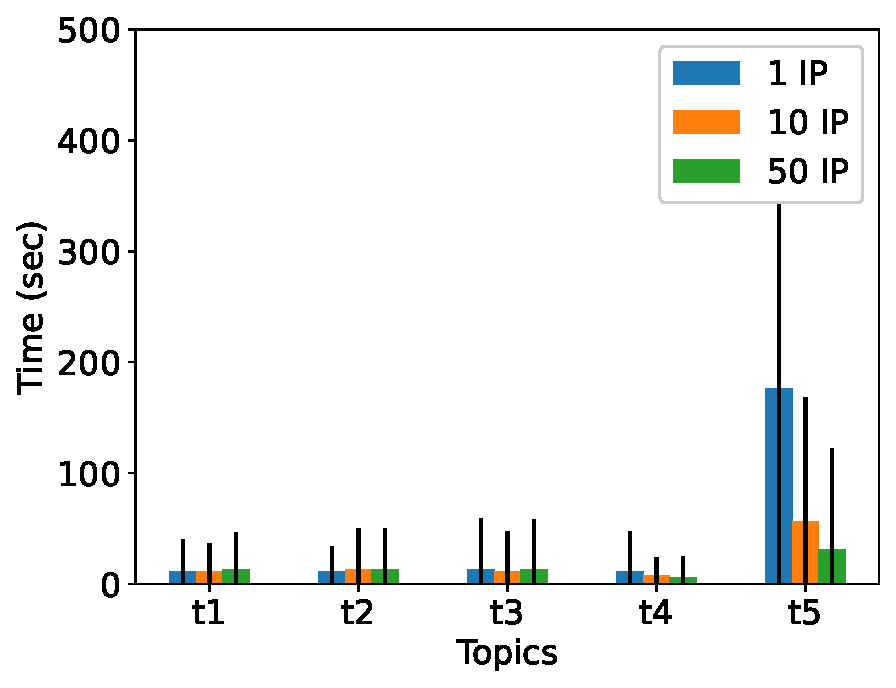
\includegraphics[width=0.225\textwidth]{img/eval/attack/min_time_discovery_t5.eps} %\hspace{-1.5em}%
\label{fig:discoverytime_eclipse_t5}
}
 \caption{Time between registration and first discovery under topic eclipsing attack} 
\label{fig:discoverytime_eclipse}
\vspace{-0.15in}
\end{figure}   

In Figure~\ref{fig:discoverytime_eclipse} we observe the average time between a node registers for a topic successfully and the node is discovered for the first time from the placed registration.
We can observe that when a topic is under attack the time required for first time discovery increases. 
This is caused by the fact that there are much more registrations in the topic caused by the attack and also that malicious nodes discovery time is higher due to the difficulty to place registrations in nodes close to the topic hash.  
We can observe that when using more IP addresses in the attack the time required to discover a node is reduced because malicious nodes are more discovered.

\begin{figure}[!h]
\centering
\subfigure[{Lookup hopcount eclipse attack t1}]{
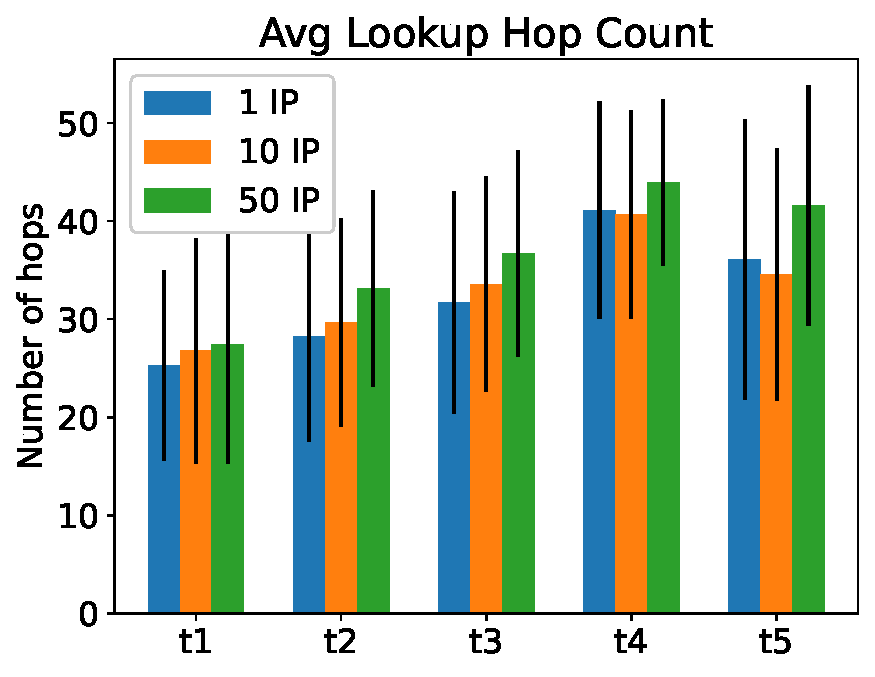
\includegraphics[width=0.225\textwidth]{img/eval/attack/lookup_hopcount_t1.eps} 
\label{fig:lookup_eclipse_t1}
} 
\hspace{-0.16cm}
\subfigure[{Lookup hopcount eclipse attack t5}]{
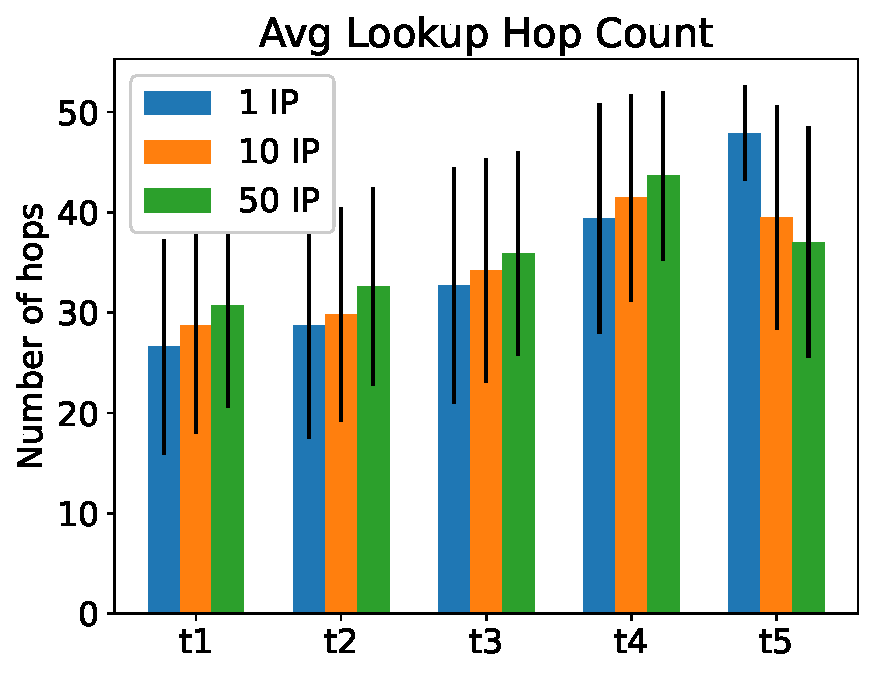
\includegraphics[width=0.225\textwidth]{img/eval/attack/lookup_hopcount_t5.eps} %\hspace{-1.5em}%
\label{fig:lookup_eclipse_t5}
}
 \caption{Lookup hopcount under topic eclipsing attack} 
\label{fig:lookup_eclipse}
\vspace{-0.15in}
\end{figure}   

\sergi{redo fig14 and fig15 figures increasing font and using eps}

In Figure~\ref{fig:lookup_eclipse} we observe the lookup hopcount in the simulation per topic,  for an eclipsing attack targeted to the most popular topic (t1) and the least popular topic (t5).
We observe that despite receiving an attack targeted at a specific topic,  the lookup performance in the network is not substantially affected by the attack.

In Figure~\ref{fig:perf_spam} we observe the performance of the topic discovery system under  the topic spam attack.
\sergi{TODO: add no sybil in the graph}
In Figure~\ref{fig:active_regs_spam} we observe the average active registrations per topic increasing the number of IP addresses used by sybil identities performing the attack.  
We observe that the number of active registrations per topic are decreased under the topic spam attack being topic 1 the most affected.
However, by observing Figure~\ref{fig:hopcount_spam} we see he lookup performance is not affected and therefore there is no substantial impact of the attack in the discovery performance of the network, concluding the system is resistant to topic spam attacks.
In Figure~\ref{fig:time_register_spam} we observe the average time required for registering for a topic,  increasing the number of Ip addresses used by sybil identities performing the attack.  
We observe again it seems there is no substantial impact of the attack to the time required to register for each topic

\sergi{add spam storage used?}

\begin{figure*}[!h]
\centering
\subfigure[{Active registrations under topic spam attack}]{
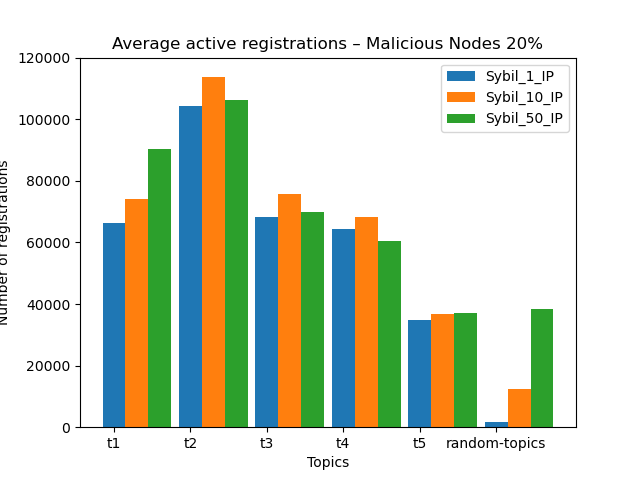
\includegraphics[width=0.275\textwidth]{img/eval/attack/registration_origin_spam.png} 
\label{fig:active_regs_spam}
} 
\hspace{-0.16cm}
\subfigure[{Time to register under topic spam attack}]{
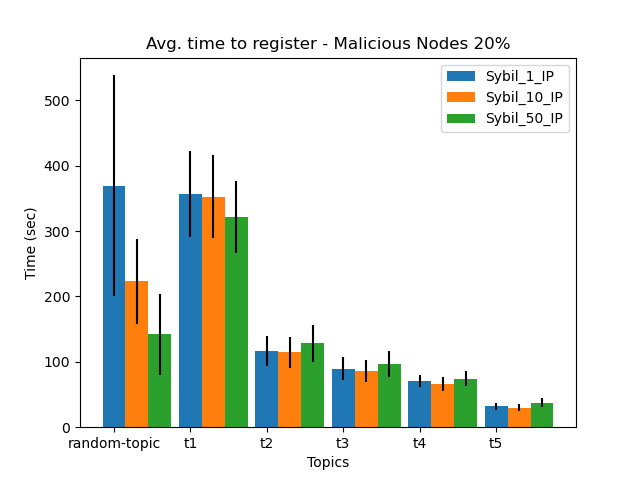
\includegraphics[width=0.275\textwidth]{img/eval/attack/avg_time_register_spam.png} %\hspace{-1.5em}%
\label{fig:time_register_spam}
}
\hspace{-0.15in}
\subfigure[{Lookup hop count topic spam attack}]{
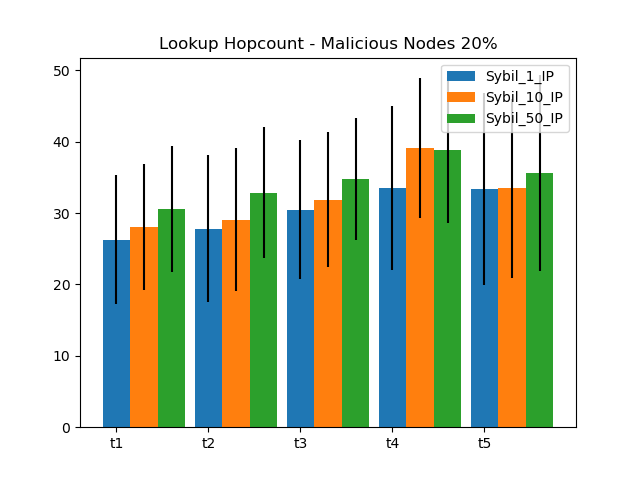
\includegraphics[width=0.275\textwidth]{img/eval/attack/lookup_hopcount_spam.png} %\hspace{-1.5em}%
\label{fig:hopcount_spam}
}
\caption{Performance evaluation topic spam attack} 
\label{fig:perf_spam}
\vspace{-0.15in}
\end{figure*}   

In Figure~\ref{fig:perf_dos} we observe the performance of the topic discovery system under the dos attack where registrars do not respond to advertisers trying to block active registrations.
In Figure~\ref{fig:active_regs_dos} we observe the average active registrations per topic increasing the number of sybil identites from 5\% to 20\% of the nodes in the network.
We observe that the number of registrations are affected by attackers,  being more affected for very popular topics,  but less affected low popularity topics.  However in none of the cases malicious nodes are able to block the active registrations and the reduction of the performance is lower than the number of sybils used.
In Figure~\ref{fig:time_register_dos} we observe the average time required for registering for a topic,  increasing the number of sybil identites from 5\% to 20\% of the nodes in the network.
We observe in this case it seems there is no substantial impact of the attack to the time required to register for each topic
In Figure~\ref{fig:time_discovery_dos} we observe the average time between an advertiser place a registration in a registrar and another node discovers it through the registrar,  increases the number sybils again.
We also observe there is no substantial impact of the attack, concluding the system is resistant to DoS attacks.

\begin{figure*}[!h]
\centering
\subfigure[{Active registrations under DoS attack}]{
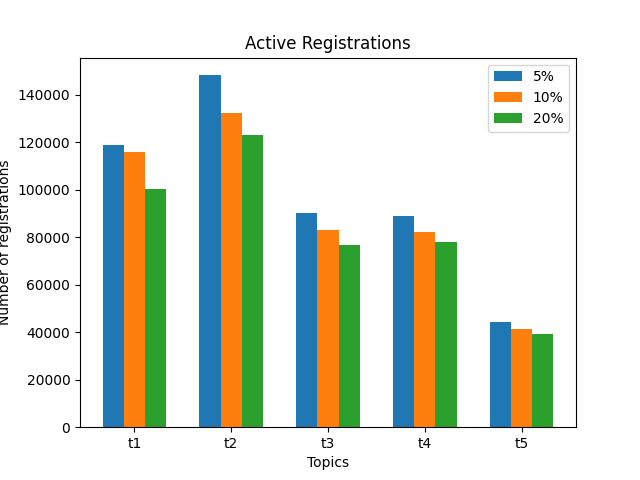
\includegraphics[width=0.275\textwidth]{img/eval/attack/registration_origin_dos.png} 
\label{fig:active_regs_dos}
} 
\hspace{-0.16cm}
\subfigure[{Time to register under DoS attack}]{
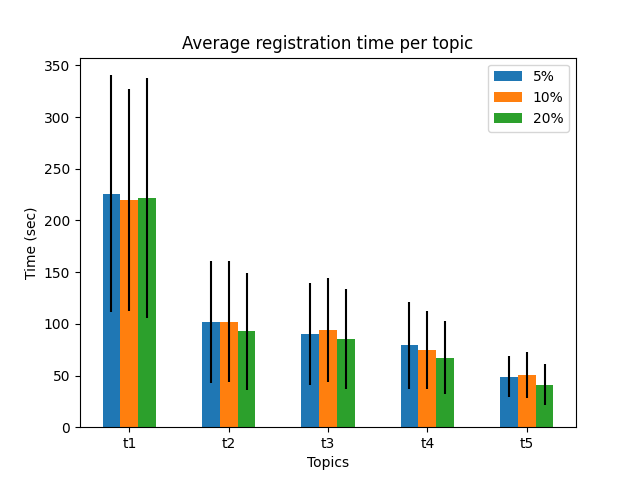
\includegraphics[width=0.275\textwidth]{img/eval/attack/avg_time_register_dos.png} %\hspace{-1.5em}%
\label{fig:time_register_dos}
}
\label{fig:discovery_dos}
\hspace{-0.15in}
\subfigure[{Time to first discovery under DoS attack}]{
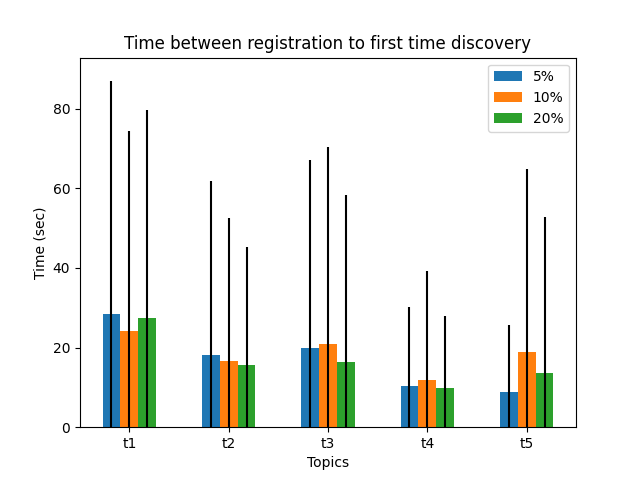
\includegraphics[width=0.275\textwidth]{img/eval/attack/min_time_discovery_dos.png} %\hspace{-1.5em}%
\label{fig:time_discovery_dos}
}
\label{fig:perf_dos}
\caption{Performance evaluation no-response DoS attack} 
\vspace{-0.15in}
\end{figure*}   

\fi
%\subsection{Testbed evaluation}
%
%"Geth"~\cite{go-ethereum} performance evaluation: \hl{TBC}.
